\documentclass{article}

% Packages
\usepackage{fancyhdr}
\usepackage{extramarks}
\usepackage{amsmath}
\usepackage{amsthm}
\usepackage{amsfonts}
\usepackage{tikz}
\usepackage[plain]{algorithm}
\usepackage{algpseudocode}
\usepackage{amssymb}
\usepackage{dsfont}
\usepackage{bbm}
\usepackage{geometry}
\usepackage{graphicx}
\usepackage{enumerate}

\usetikzlibrary{automata,positioning}

% Document Layout
\topmargin=-0.45in
\evensidemargin=0in
\oddsidemargin=0in
\textwidth=6.5in
\textheight=9.0in
\headsep=0.25in
\linespread{1.1}

% Page Style
\pagestyle{fancy}
\lhead{\hmwkAuthorName}
\chead{\hmwkClass:\ \hmwkTitle}
\rhead{Section \hmwkSection, \firstxmark}
\lfoot{\lastxmark}
\cfoot{\thepage}
\renewcommand\headrulewidth{0.4pt}
\renewcommand\footrulewidth{0.4pt}

% Paragraph Settings
\setlength\parindent{0pt}
\setlength{\parskip}{5pt}

% Section Management
\newcommand{\hmwkSection}{A} % Current section (A, B, or C) - update manually

% Problem Header Management
\newcommand{\enterProblemHeader}[1]{
  \nobreak\extramarks{}{Problem \arabic{#1} continued on next page\ldots}\nobreak{}
  \nobreak\extramarks{Problem \arabic{#1} (continued)}{Problem \arabic{#1} continued on next page\ldots}\nobreak{}
}

\newcommand{\exitProblemHeader}[1]{
  \nobreak\extramarks{Problem \arabic{#1} (continued)}{Problem \arabic{#1} continued on next page\ldots}\nobreak{}
  \stepcounter{#1}
  \nobreak\extramarks{Problem \arabic{#1}}{}\nobreak{}
}

% Counters
\setcounter{secnumdepth}{0}
\newcounter{partCounter}
\newcounter{homeworkProblemCounter}
\setcounter{homeworkProblemCounter}{1}
\nobreak\extramarks{Problem \arabic{homeworkProblemCounter}}{}\nobreak{}

% Homework Problem Environment
% Optional argument adjusts problem counter for non-sequential problems
\newenvironment{homeworkProblem}[1][-1]{
  \ifnum#1>0
    \setcounter{homeworkProblemCounter}{#1}
  \fi
  \section{Problem \arabic{homeworkProblemCounter}}
  \setcounter{partCounter}{1}
  \enterProblemHeader{homeworkProblemCounter}
}{
  \exitProblemHeader{homeworkProblemCounter}
}

% Assignment Details
\newcommand{\hmwkTitle}{Sheet\ \#3}
\newcommand{\hmwkDueDate}{February 21, 2026}
\newcommand{\hmwkClass}{C5.4 Networks}
\newcommand{\hmwkClassInstructor}{Professor R. Lambiotte}
\newcommand{\hmwkAuthorName}{\textbf{Ray Tsai}}

% Title Page
\title{
  \vspace{2in}
  \textmd{\textbf{\hmwkClass:\ \hmwkTitle}}\\
  \normalsize\vspace{0.1in}\small{Due\ on\ \hmwkDueDate\ at 12:00pm}\\
  \vspace{0.1in}\large{\textit{\hmwkClassInstructor}} \\
  \vspace{3in}
}

\author{\hmwkAuthorName}
\date{}

% Part Command
\renewcommand{\part}[1]{\textbf{\large Part \Alph{partCounter}}\stepcounter{partCounter}\\}

% Mathematical Commands
% Algorithms
\newcommand{\alg}[1]{\textsc{\bfseries \footnotesize #1}}

% Calculus
\newcommand{\deriv}[1]{\frac{\mathrm{d}}{\mathrm{d}x} (#1)}
\newcommand{\pderiv}[2]{\frac{\partial}{\partial #1} (#2)}
\newcommand{\dx}{\mathrm{d}x}

% Probability and Statistics
\newcommand{\Var}{\mathrm{Var}}
\newcommand{\Cov}{\mathrm{Cov}}
\newcommand{\Bias}{\mathrm{Bias}}
\newcommand*{\prob}{\mathbb{P}}
\newcommand*{\E}{\mathbb{E}}

% Number Sets
\newcommand*{\Z}{\mathbb{Z}}
\newcommand*{\Q}{\mathbb{Q}}
\newcommand*{\R}{\mathbb{R}}
\newcommand*{\C}{\mathbb{C}}
\newcommand*{\N}{\mathbb{N}}

\begin{document}

\maketitle
\pagebreak

\begin{homeworkProblem}
  \begin{enumerate}[(a)]
    \item In the Louvain method, the efficiency of the algorithm partly resides in the fact that the variation of modularity $\Delta_{ij}$ obtained by moving a vertex $i$ from its community to the community of one of its neighbors $j$ can be calculated with only local information. In practice, the variation of modularity is calculated by removing $i$ from its community $\Delta_{remove;i}$ (this is only done once) then inserting it into the community of $j$ $\Delta_{insert;ij}$ for each neighbor $j$ of $i$. The variation is therefore: $\Delta_{ij} = \Delta_{remove;i} + \Delta_{insert;ij}$. Derive analytically $\Delta_{remove;i}$ when removing node $i$ from its community $C_i$.

    \item Show that if a partition contains a disconnected community, it is always preferable (in terms of modularity) to split this community into connected communities.

    \item Despite the previous result, is it possible that the Louvain method produces communities that do not form connected components?
    
    Download the DBLP collaboration network ($n \approx 317\,000$ nodes, $m \approx 1\,050\,000$ edges, available from the SNAP repository). Run Louvain on this network for several random seeds and report the number of disconnected and badly connected communities.
    
    This point is discussed in \texttt{https://arxiv.org/pdf/1810.08473.pdf} (see Figure 2).
\end{enumerate}
\end{homeworkProblem}

\newpage

% To change sections, use: \renewcommand{\hmwkSection}{B}
% Example: Uncomment the line below when you start Section B
\renewcommand{\hmwkSection}{B}

\begin{homeworkProblem}
  \begin{enumerate}[(a)]
    \item Show that the combinatorial graph Laplacian $L = D - A$ is positive semi-definite. More precisely, show that for any vector $v \in \mathbb{R}^n$,
    \[
    v^T L v = \sum_{(i,j) \in E} (v_i - v_j)^2 \geq 0.
    \]
    Deduce that $\lambda_1 = 0$ is the smallest eigenvalue and that its eigenvector is proportional to $\mathbf{1} = (1, 1, \dots, 1)^T$.

    \begin{proof}
      Since
      \[
        v^TLv = v^TDv - v^TAv = \sum_{i = 1}^n v_i^2 d_i - \sum_{(i,j) \in E} 2v_i v_j = \sum_{(i,j) \in E} v_i^2 - 2v_i v_j + v_j^2 = \sum_{(i,j) \in E} (v_i - v_j)^2 \geq 0.
      \]
      $L$ is positive semi-definite, and so its eigenvalues $0 = \lambda_1 \leq \lambda_2 \leq \cdots \leq \lambda_n$ are non-negative. Write $\mathbf{1} = \sum_{i = 1}^n c_i u_i$ for some $c_i \in \R$, where $u_i$ are the normalized eigenvectors of $L$. But then 
      \[
        0 = \mathbf{1}^TL\mathbf{1} = \sum_{i = 1}^n c_i^2\lambda_i,
      \]
      so $\lambda_1 = 0$ and $\mathbf{1}$ is its corresponding eigenvector.
    \end{proof}

    \item Consider the \textbf{expected adjacency matrix} $\bar{A} = \mathbb{E}[A]$ of the symmetric two-community SBM with $n_1 = n_2 = n/2$. This is the $n \times n$ matrix with $\bar{A}_{ij} = p_{in}$ if nodes $i, j$ are in the same community, and $\bar{A}_{ij} = p_{out}$ otherwise (with $\bar{A}_{ii} = 0$).

    \begin{enumerate}[i.]
      \item Show that $\bar{A}$ has rank 2 (ignoring the zero diagonal correction). \textit{Hint: write $\bar{A}$ as a sum of two outer products involving the vectors $\mathbf{1}$ and $u$, where $u_i = +1$ for community 1, $u_i = -1$ for community 2.}
      \begin{proof}
        Note that 
        \[
          \bar{A} = \frac{p_{in} + p_{out}}{2}\mathbf{1}\mathbf{1}^T + \frac{p_{in} - p_{out}}{2}u u^T,
        \]
        which is the sum of two linearly independent rank-1 matrices, so $\bar{A}$ has rank 2.
      \end{proof}
      \item Compute the two non-zero eigenvalues of $\bar{A}$.
      \begin{proof}
        Since $u$ has equal number of $+1$s and $-1$s, we have $\mathbf{1}^Tu = 0$. Thus,
        \[
          \bar{A}\mathbf{1} = \frac{p_{in} + p_{out}}{2}\mathbf{1}\mathbf{1}^T\mathbf{1} = \frac{p_{in} + p_{out}}{2}n\mathbf{1},
        \]
        \[
          \bar{A}u = \frac{p_{in} - p_{out}}{2}uu^Tu = \frac{p_{in} - p_{out}}{2}nu.
        \]
      \end{proof}
      \item Form $\bar{L} = \bar{D} - \bar{A}$ where $\bar{D} = \text{diag}(\bar{A}\mathbf{1})$. Show that the second eigenvector of $\bar{L}$ (the ``Fiedler vector'' of the expected graph) is exactly the community indicator $u$. Find $\lambda_2(\bar{L})$ as a function of $c_{in}$ and $c_{out}$.
      \begin{proof}
        Since every node has the same expected degree, $\bar{D} = (c_{in} + c_{out})I$. Thus $\bar{L}\mathbf{1} = 0$ and
        \[
          \bar{L}u = \bar{D}u - \bar{A}u = (c_{in} + c_{out})u - \frac{p_{in} - p_{out}}{2}nu =2c_{out}u.
        \]
        Note that any eigenvector $v$ other than $\mathbf{1}$ and $u$ is orthogonal to both $\mathbf{1}$ and $u$, so $Av = 0$. Thus, 
        \[
          \bar{L}v = \bar{D}v - \bar{A}v = (c_{in} + c_{out})v.
        \]
        Thus, the second eigenvector of $\bar{L}$ is $u$.
      \end{proof}
    \end{enumerate}

    \item Generate SBM graphs with $n_1 = n_2 = 100$ and $p_{in} = 0.1$. For each value of $p_{out}/p_{in} \in \{0, 0.05, 0.10, \dots, 1.0\}$, generate 20 independent realisations. For each graph:
    \begin{enumerate}[i.]
      \item Compute the Fiedler vector of the combinatorial Laplacian $L = D - A$.
      \item Classify each node into community 1 or 2 by the sign of its Fiedler vector entry.
      \item Report the \textbf{classification accuracy} (fraction of correctly classified nodes, taking the better of the two label assignments).
    \end{enumerate}
    Plot the mean accuracy (with error bars) as a function of $p_{out}/p_{in}$. At what ratio does the Laplacian start to fail?

    \begin{center}
      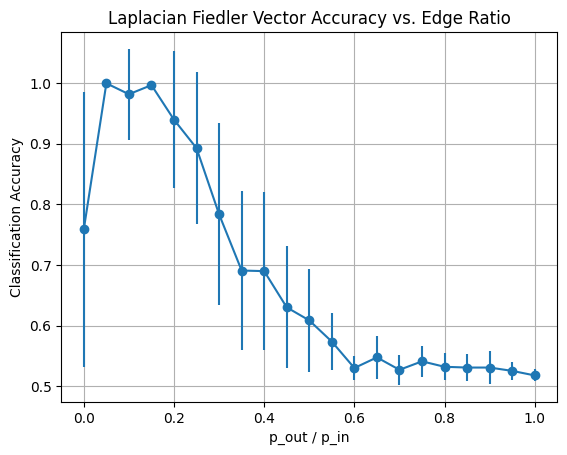
\includegraphics[width=0.8\textwidth]{./images/acc.png}
    \end{center}

    \item The \textbf{normalised Laplacian} is
    \[
    \mathcal{L} = D^{-1/2} L D^{-1/2} = I - D^{-1/2} A D^{-1/2}.
    \]
    Show that all eigenvalues of $\mathcal{L}$ lie in the interval $[0, 2]$.
    
    \textit{Hint: relate $\mathcal{L}$ to the random walk transition matrix $T = D^{-1} A$ and use the fact that $T$ is a row-stochastic matrix with eigenvalues in $[-1, 1]$.}

    \begin{proof}
      Note that $D^{1/2} T D^{-1/2} = D^{-1/2} A D^{-1/2}$. But then $T$ and $D^{-1/2} A D^{-1/2}$ are similar matrices, so they share the same eigenvalues. Since $T$ is a row stochastic matrix, its eigenvalues lie in $[-1, 1]$. Thus, the eigenvalues of $\mathcal{L}$ lie in $[0, 2]$.
    \end{proof}
\end{enumerate}
\end{homeworkProblem}

\end{document}